\section{Solution \#3:}

\subsection{Core Activities of this Solution}

\begin{itemize}
	\item selecting a diet
	
	\item scanning products
\end{itemize}

\subsection{The Reason for Prototype Selection}

We summarized our ideas and concluded them in one solution. We choosed paper prototype again because it fitted our problem.

\subsection{Prototyping Process Explained}

First, we identified core activities. Then we had a brainstorm about possible screens. We choosed possible ways of the user interaction. Those are:
\begin{itemize}
	\item menu with diet selection\\
	(\autoref{s3:menu})
	
	\begin{enumerate}
		\item vegeterian
     	(\autoref{s3:vege})
    	\item keto
    	(\autoref{s3:keto})
    	\item no constraints
    	(\autoref{s3:nocons})
	\end{enumerate}
   	
   	\item summaries
   	\begin{enumerate}
		\item summary of vegeterian diet
     	(\autoref{s3:sumvege})
    	\item summary of keto diet
    	(\autoref{s3:sumketo})
    	\item summary of diet with no constraints
    	(\autoref{s3:sumnocons})
	\end{enumerate}
	
\end{itemize}

\clearpage
\subsection{Prototype Itself}

\begin{figure}[H]
	\centering
	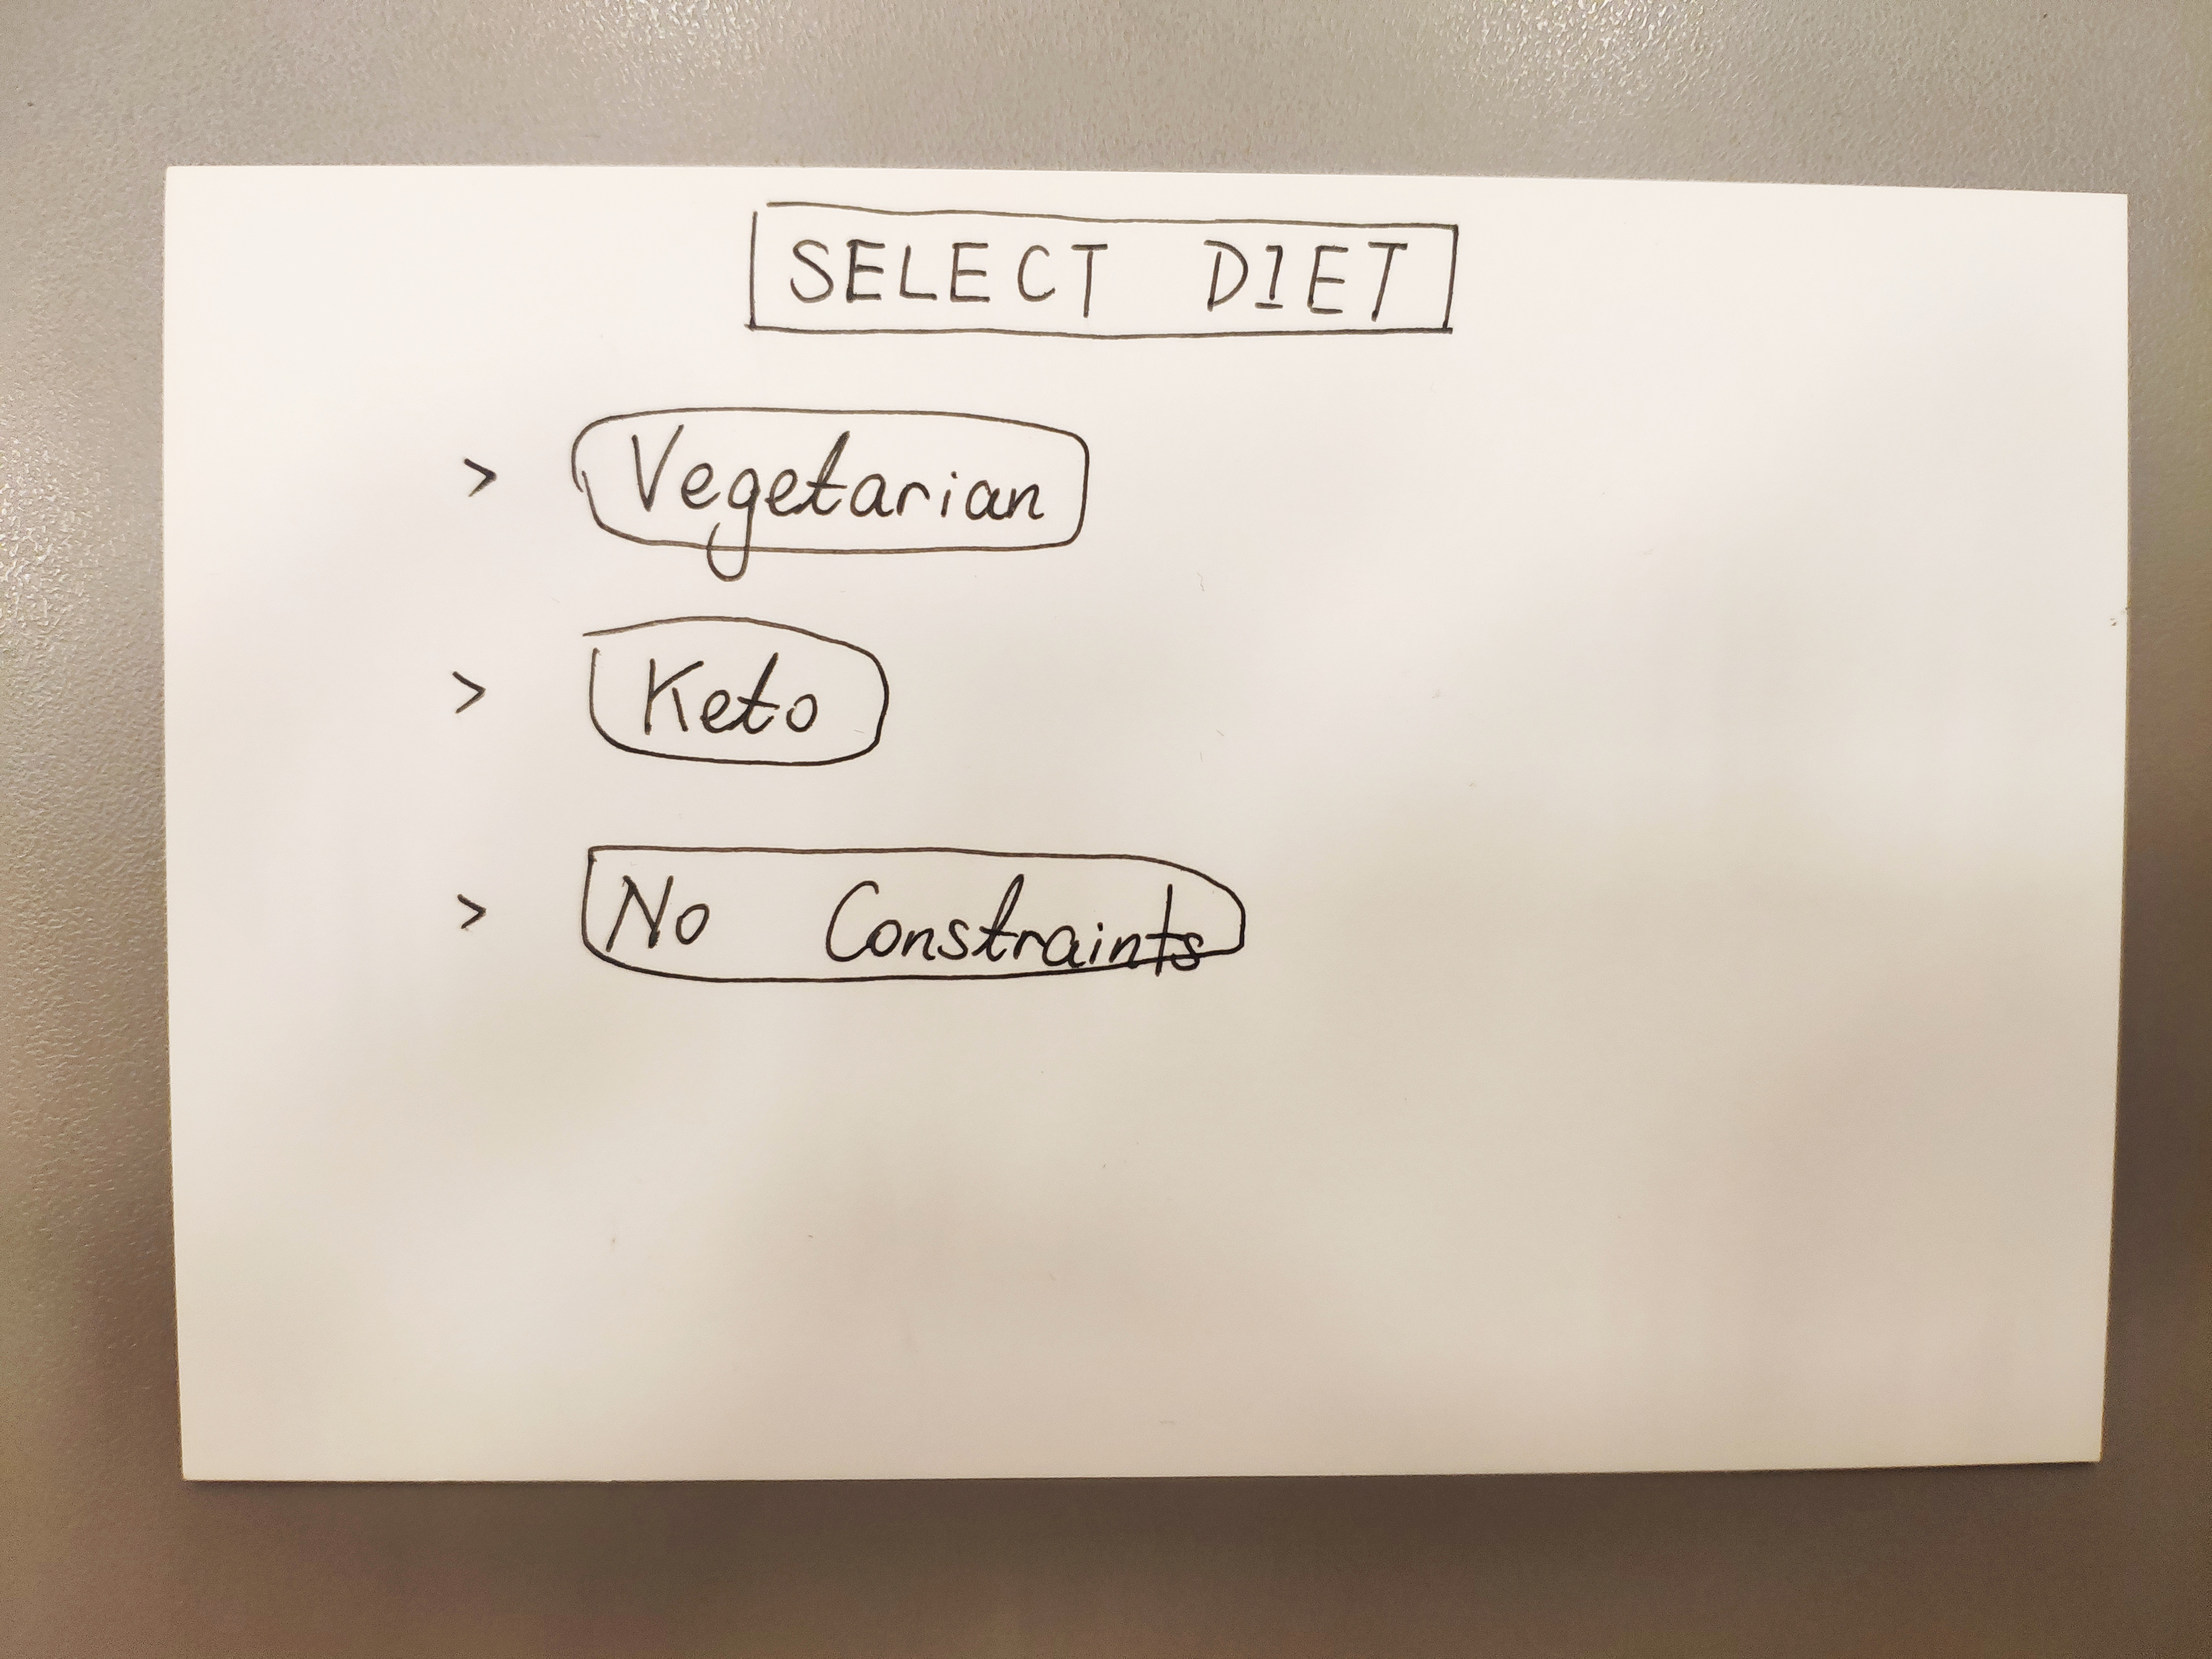
\includegraphics[trim={10em 10em 10em 10em},  clip, width=0.80\textwidth]{images/s3/1.jpg}
	\caption{ User chooses one of three diets }
	\label{s3:menu}
\end{figure}

\begin{figure}[H]
	\centering
	\includegraphics[trim={10em 10em 10em 10em}, clip, width=0.80\textwidth]{images/s3/4.jpg}
	\caption{ Screen of vegetarian diet }
	\label{s3:vege}
\end{figure}

\begin{figure}[H]
	\centering
	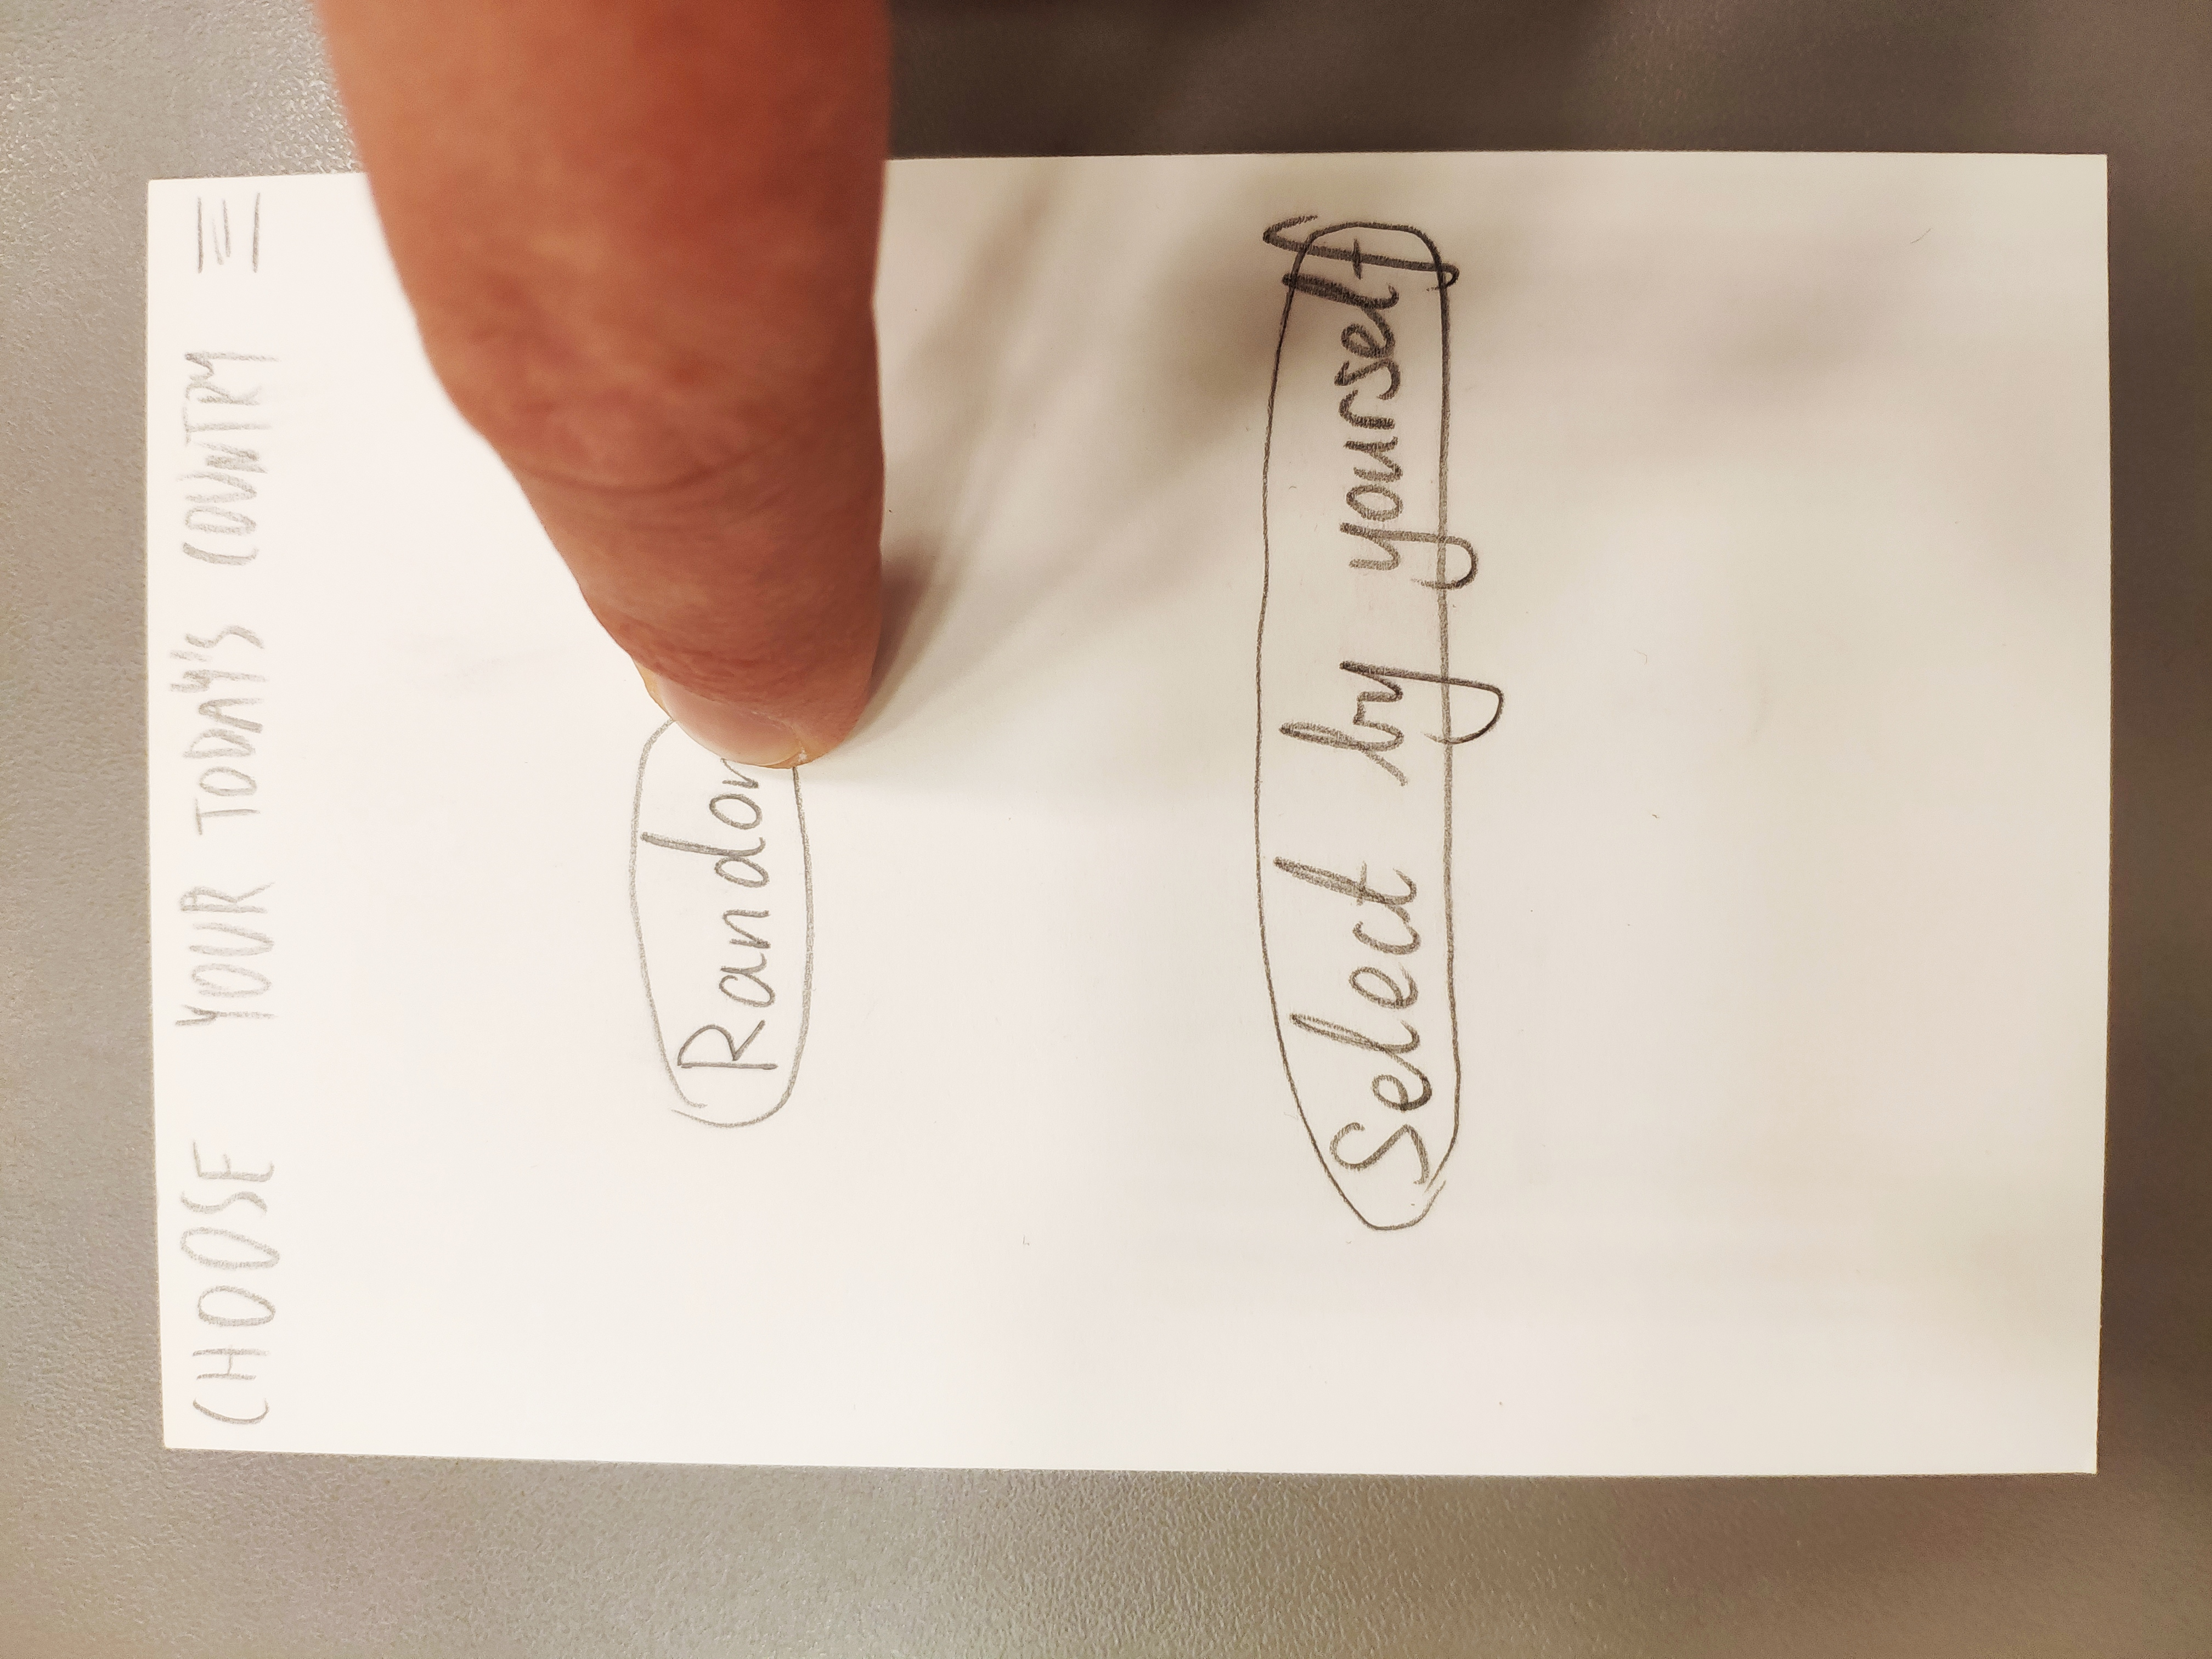
\includegraphics[trim={10em 10em 10em 10em}, clip, width=0.8\textwidth]{images/s3/7.jpg}
	\caption{ Screen of keto diet }
	\label{s3:keto}
\end{figure}

\begin{figure}[H]
	\centering
	\includegraphics[trim={10em 10em 10em 10em}, clip, width=0.8\textwidth]{images/s3/10.jpg}
	\caption{ Screen of diet with no constraints }
	\label{s3:nocons}
\end{figure}

\begin{figure}[H]
	\centering
	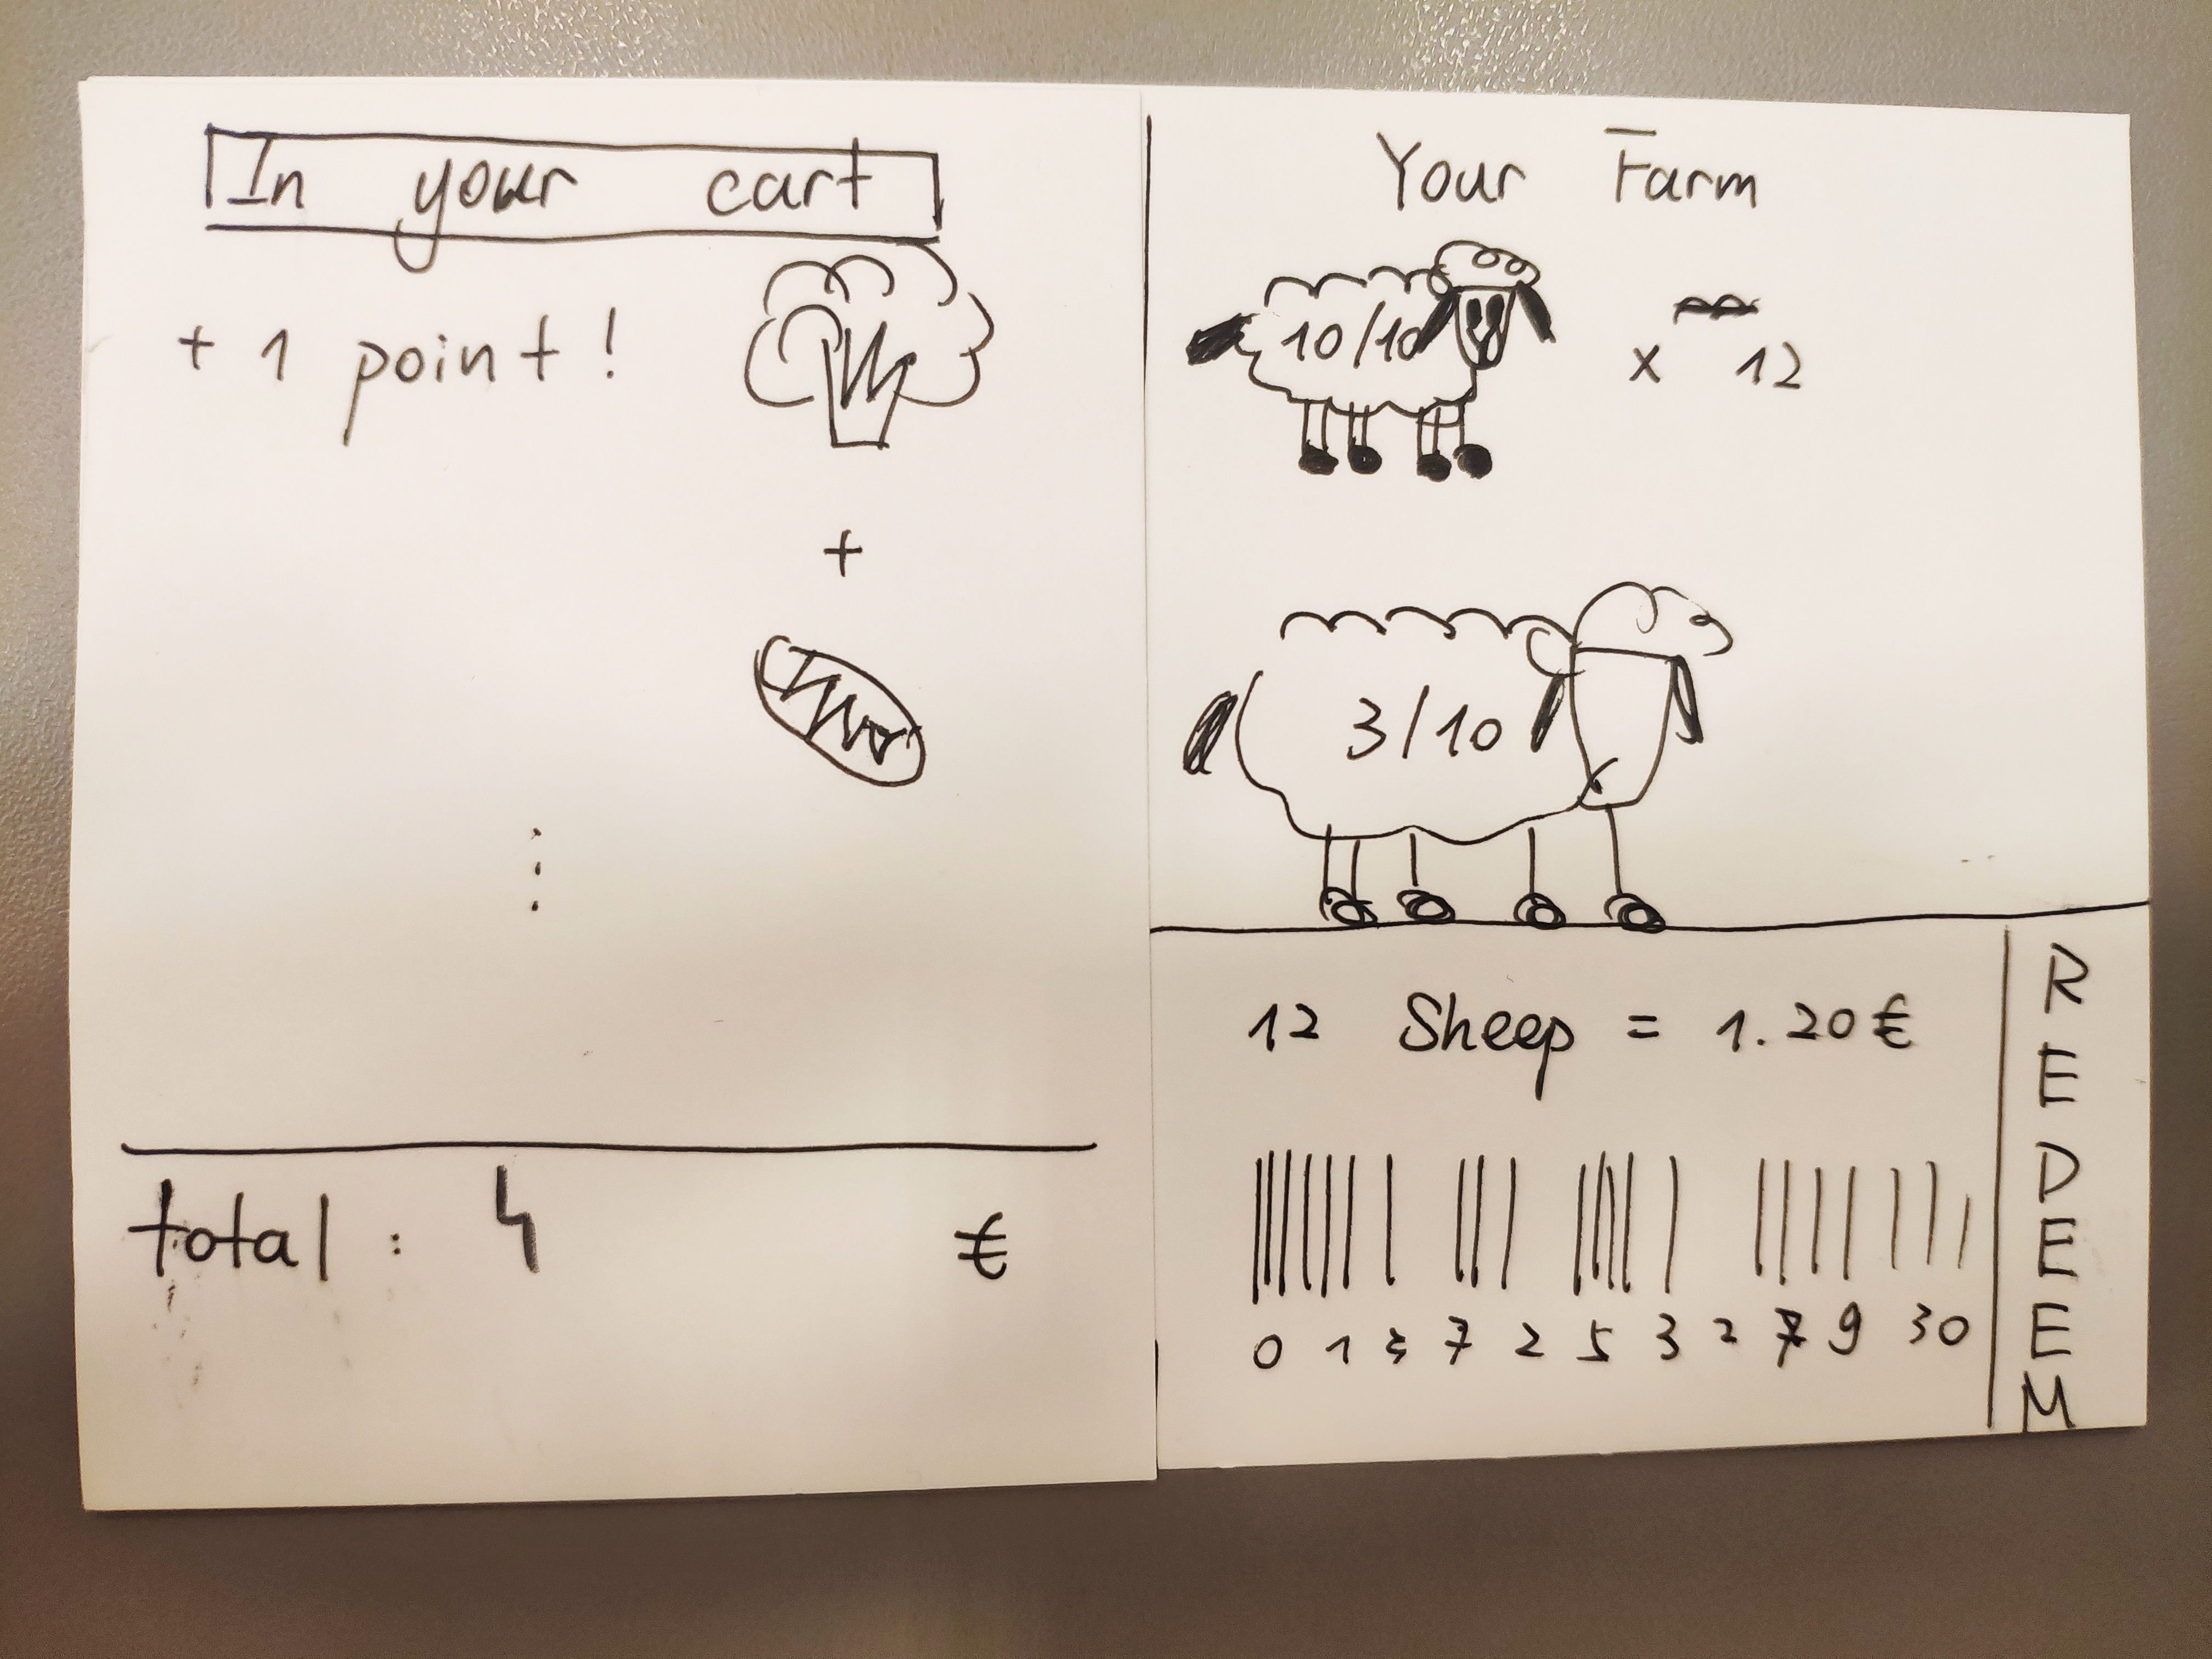
\includegraphics[trim={10em 10em 10em 10em}, clip, width=0.8\textwidth]{images/s3/5.jpg}
	\caption{ Summary of vegetarian diet }
	\label{s3:sumvege}
\end{figure}

\begin{figure}[H]
	\centering
	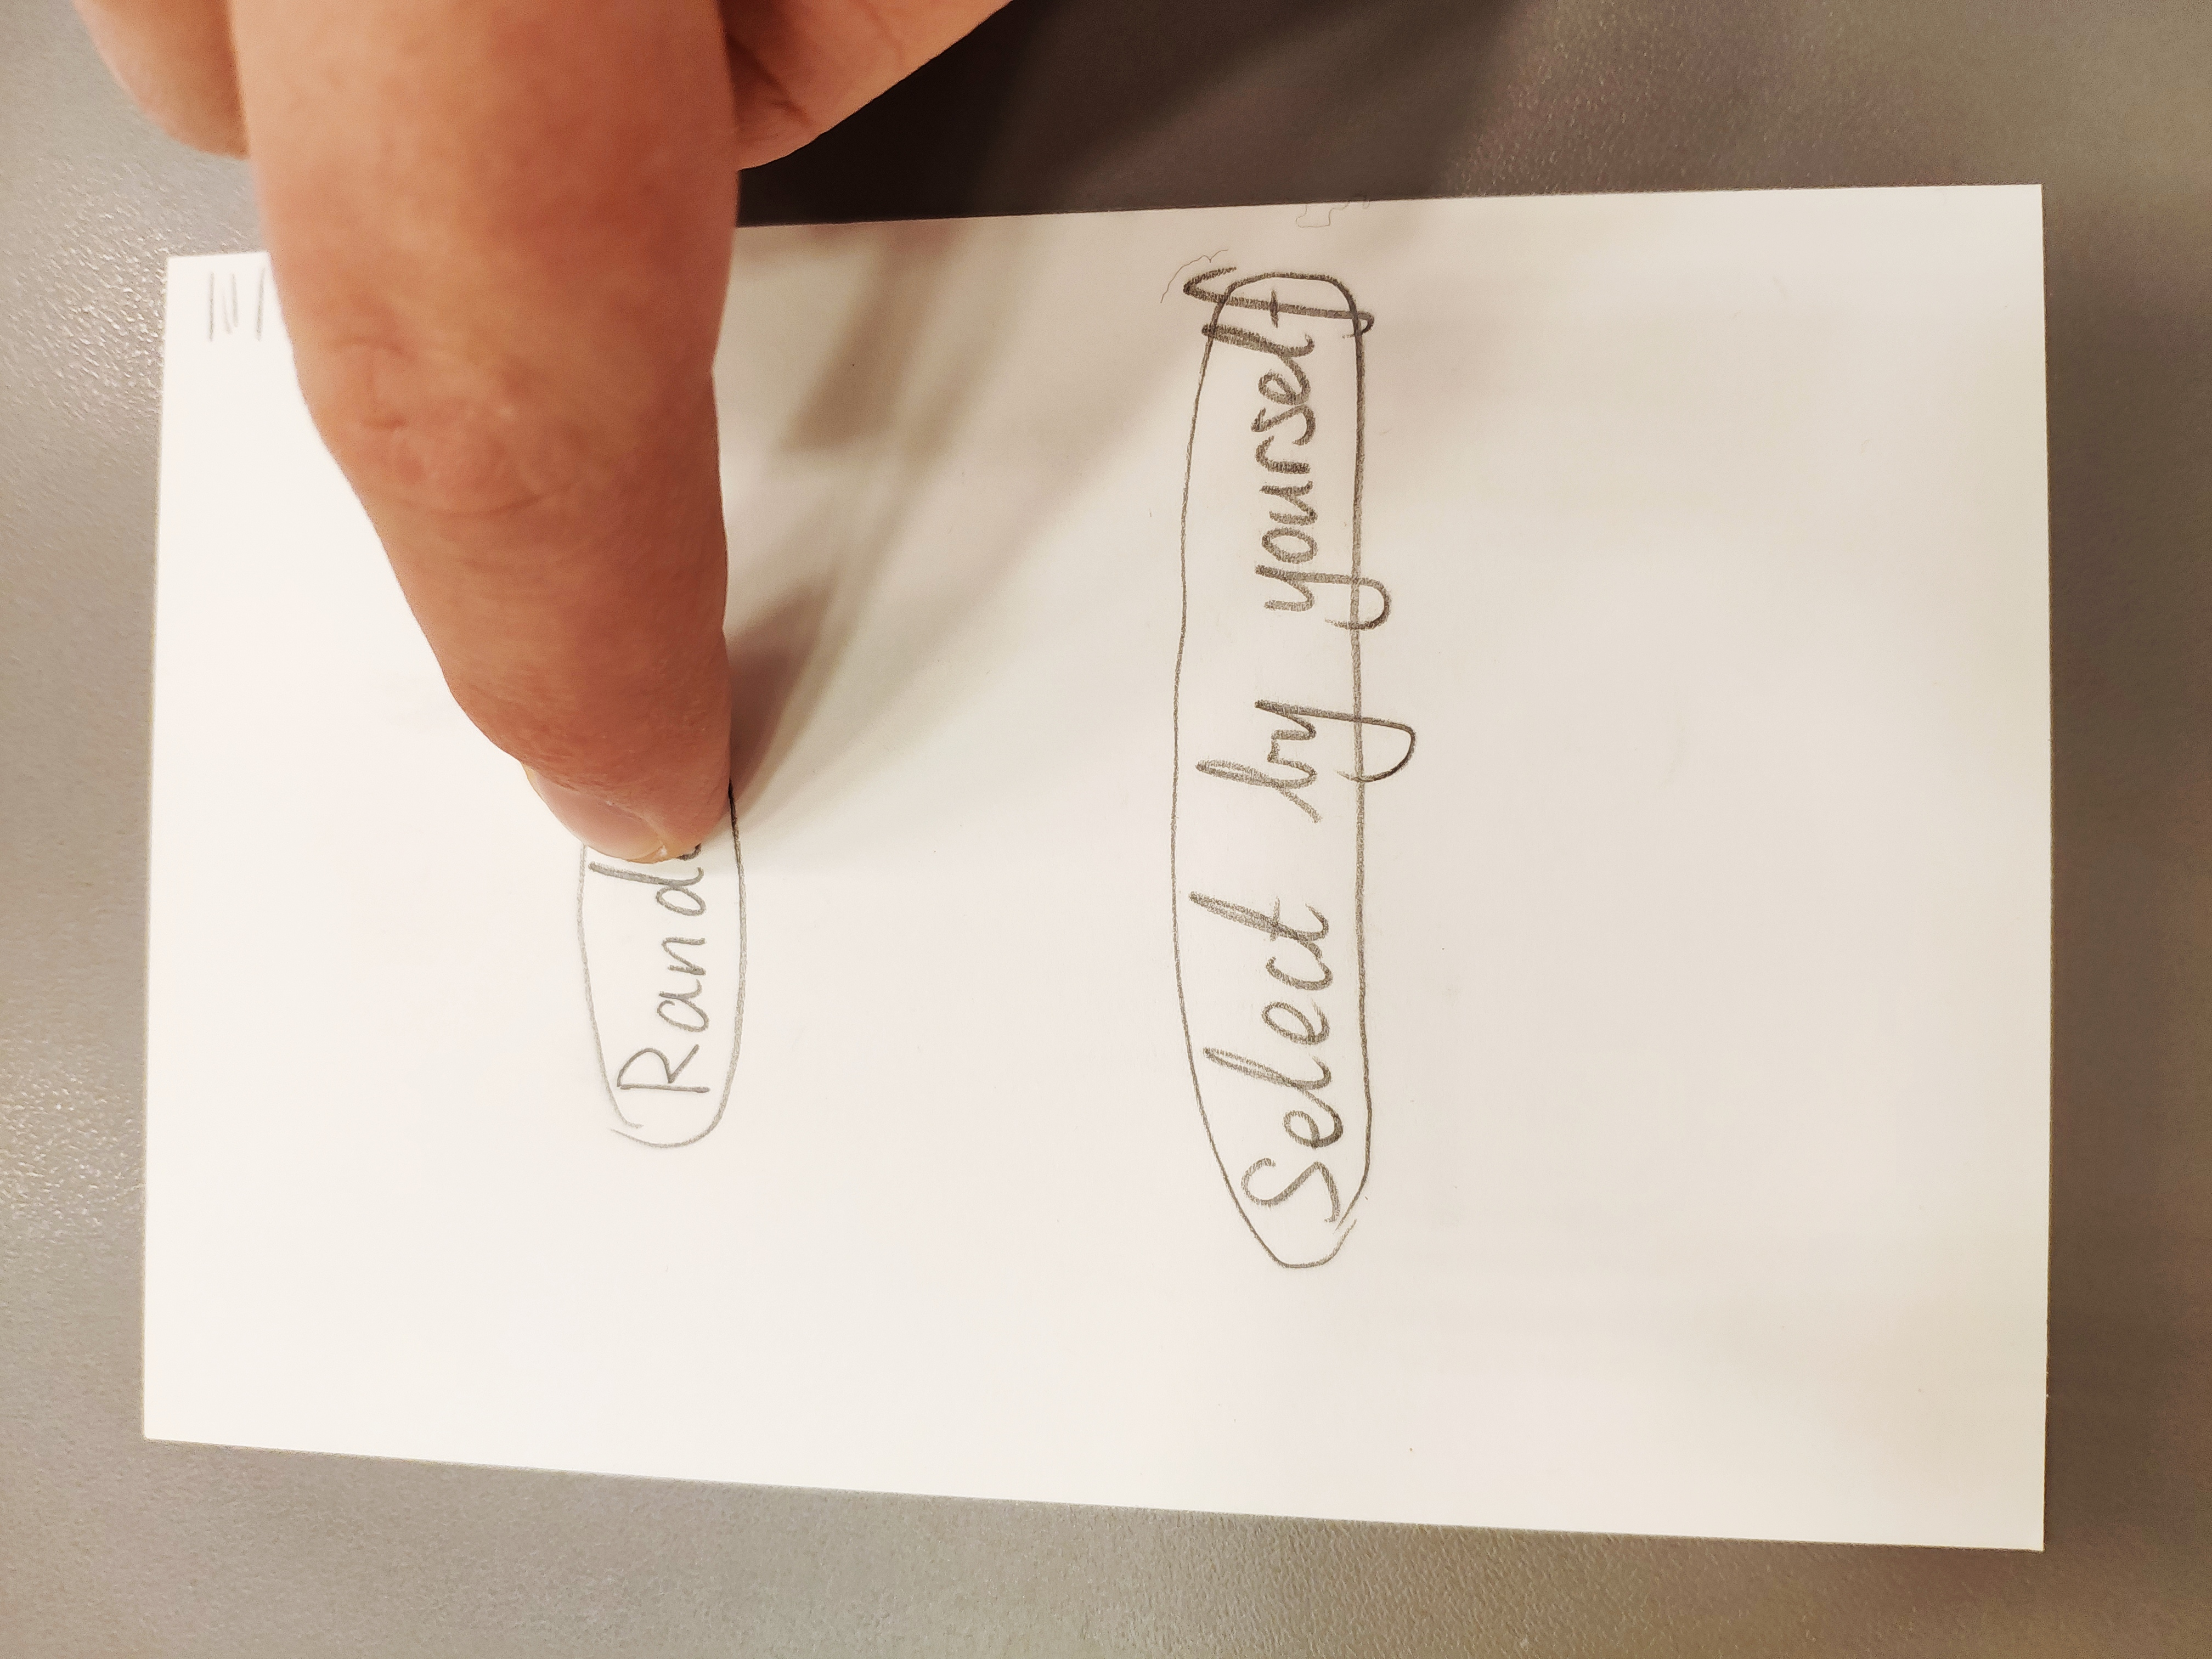
\includegraphics[trim={10em 10em 10em 10em}, clip, width=0.8\textwidth]{images/s3/8.jpg}
	\caption{ Summary of keto diet }
	\label{s3:sumketo}
\end{figure}


\begin{figure}[H]
	\centering
	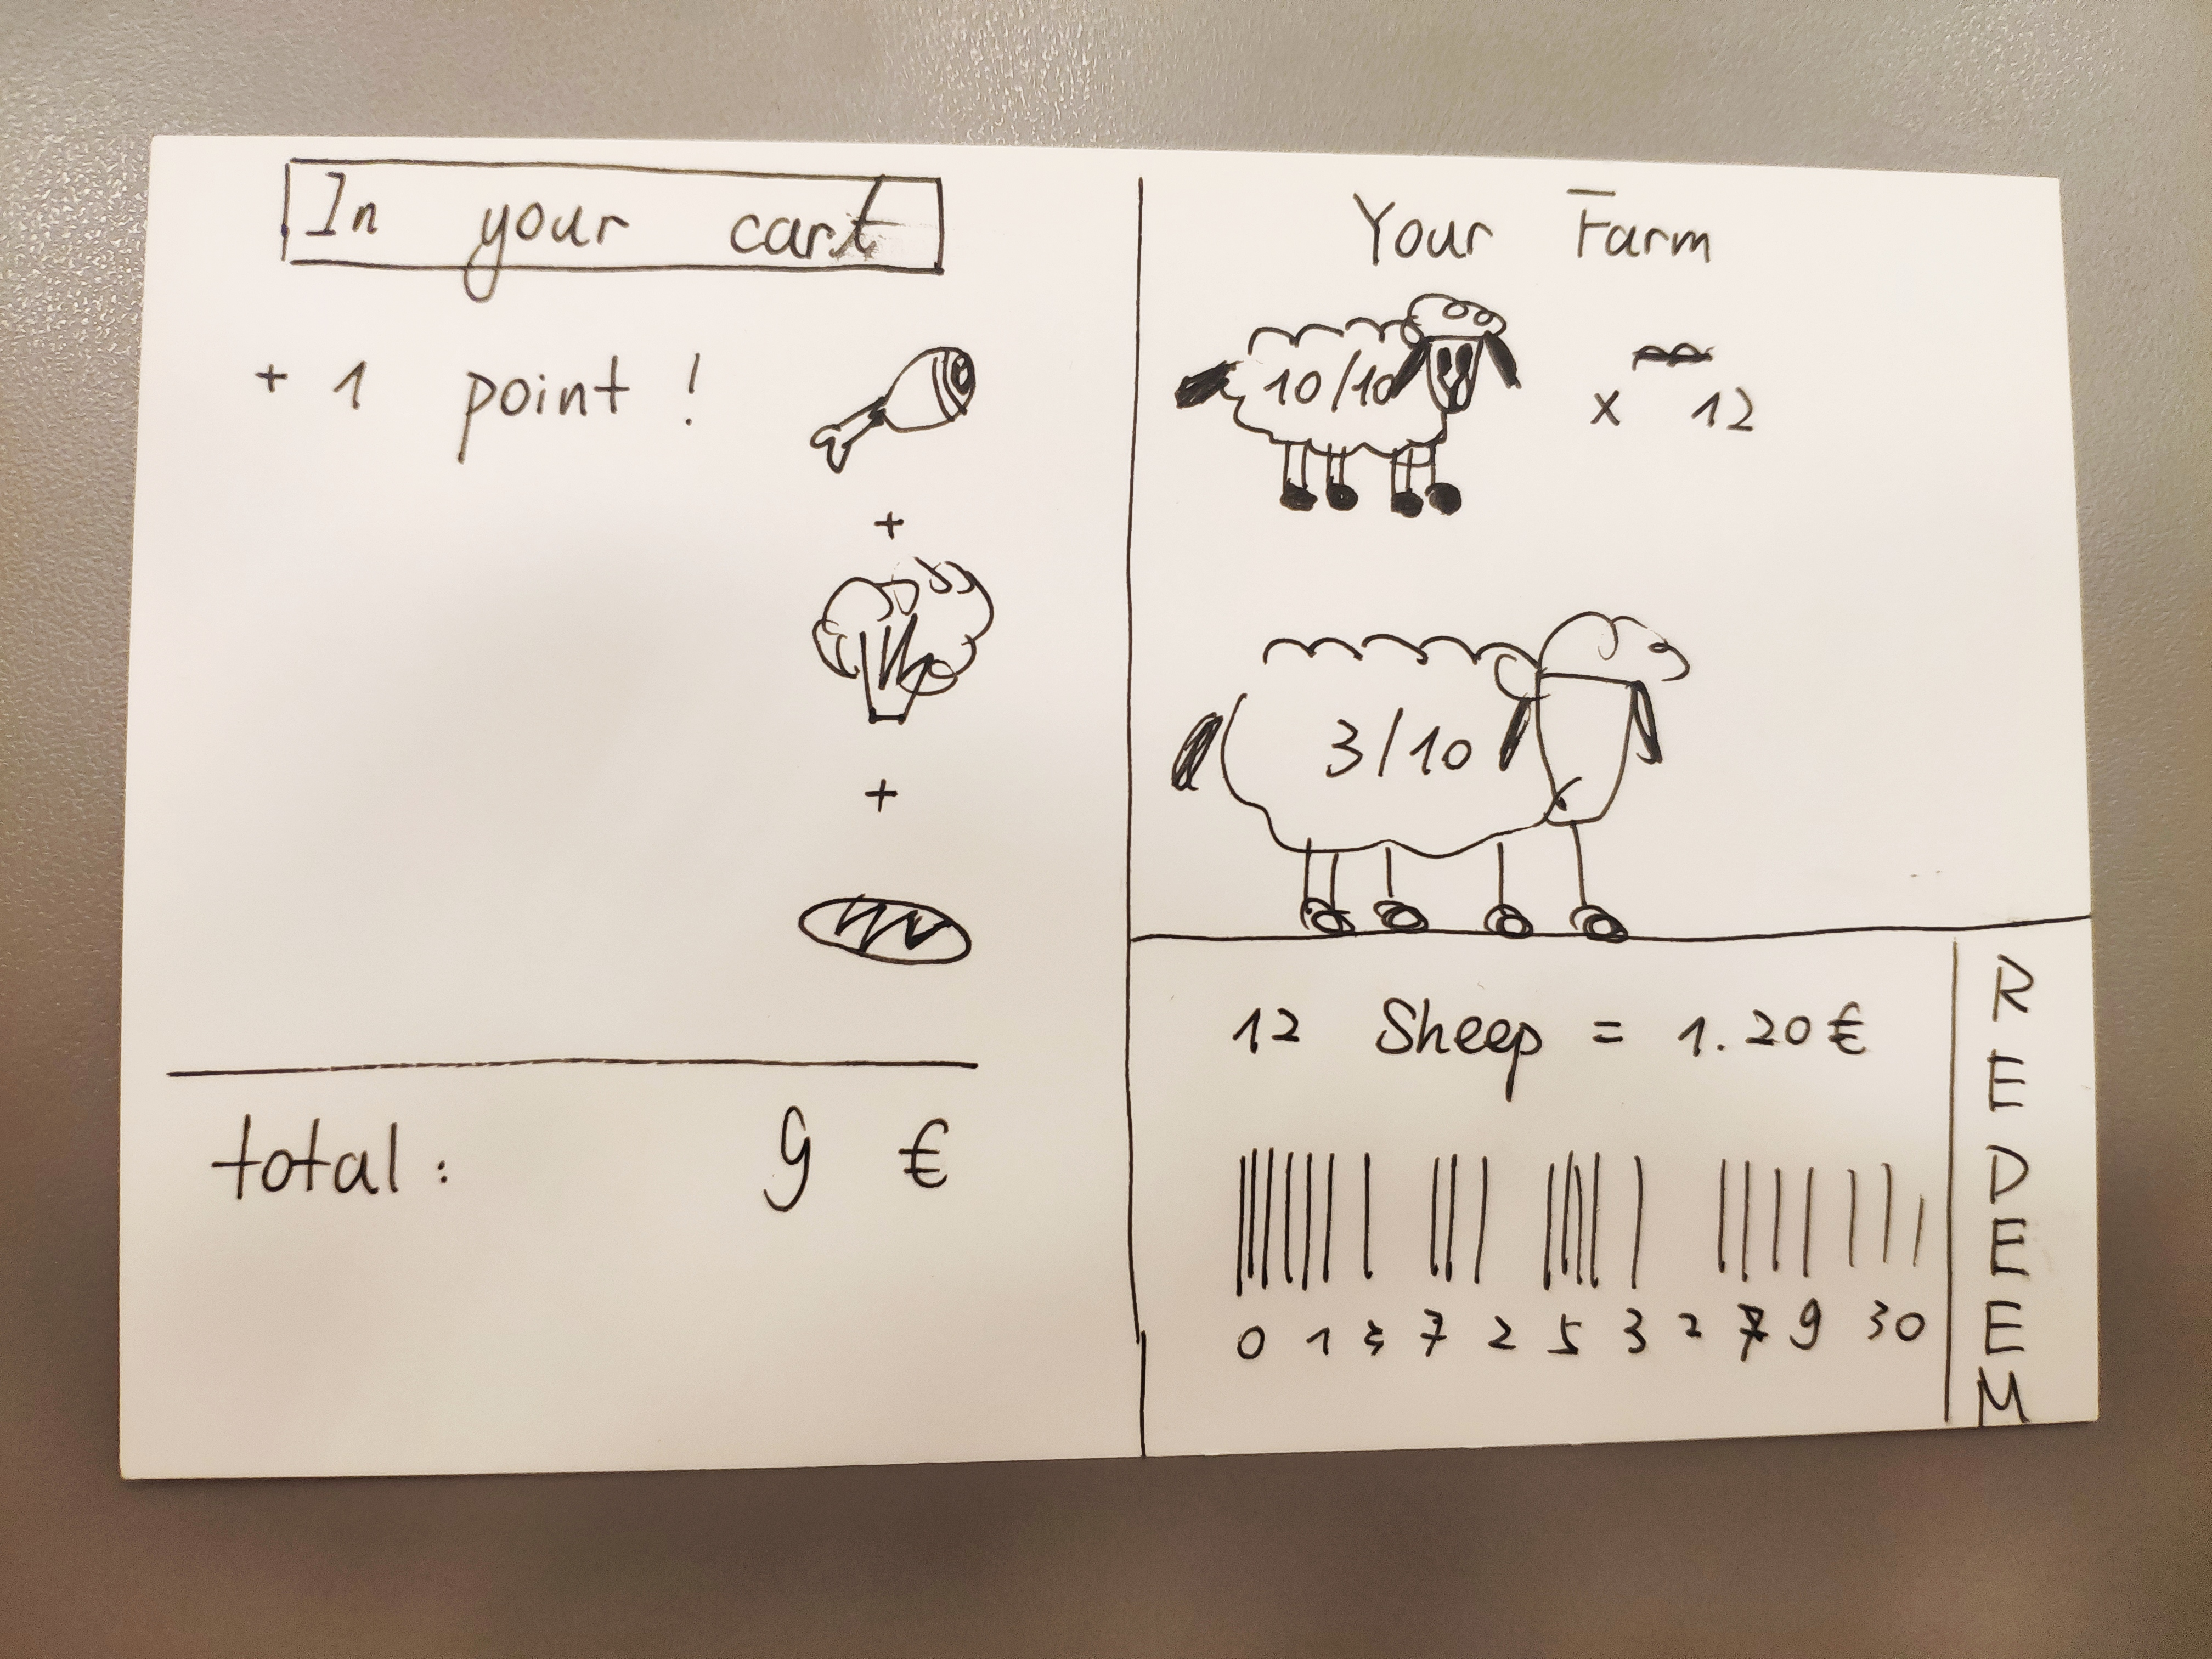
\includegraphics[trim={10em 10em 10em 10em}, clip, width=0.8\textwidth]{images/s3/11.jpg}
	\caption{ Summary of diet with no constraints }
	\label{s3:sumnocons}
\end{figure}